\documentclass[10pt,a4paper]{beamer}
\usepackage[utf8]{inputenc}
\usepackage[T1]{fontenc}
\usepackage{hyperref}
\usepackage[english]{babel}
\usepackage{hyperref}
\usepackage{amssymb,amsthm,amsmath,amsfonts}
\usepackage{lmodern}
\usepackage{units}
\usepackage{hyperref}
\usepackage{tikz}
\usetikzlibrary{calc}
\usetikzlibrary{fixedpointarithmetic}
\usepackage{fp}
\usepackage{graphicx}
\bibliographystyle{plain}
\usepackage{epsfig}
\usepackage{epstopdf}
\usepackage{makeidx}
\usepackage{gloss}
\usepackage{algorithmic}
\usepackage{algorithm}

\usepackage{xkeyval} 

\def\glossname{Glossaire}
%\bibliographystyle{alpha} % plain-fr si rapport en français

\usepackage[usenames,dvipsnames]{pstricks}
\usepackage{epsfig}
\usepackage{pst-grad} % For gradients
\usepackage{pst-plot}



\theoremstyle{plain}
\newtheorem{thm}{Theorem}[part]
\theoremstyle{definition} 
\newtheorem{lem}[thm]{Lemma}
\theoremstyle{definition} 
\newtheorem{cor}[thm]{Corollary}
\theoremstyle{definition} 
\newtheorem{prop}[thm]{Proposition}
\theoremstyle{definition} 
\newtheorem{defi}[thm]{Definition}
\theoremstyle{remark} 
\newtheorem{rem}[thm]{Remark}
\theoremstyle{remark} 
\newtheorem{exe}[thm]{Example}

\useoutertheme{split}
\useinnertheme{rounded}
\usecolortheme{whale}
\usecolortheme{orchid}
\usecolortheme[named=orange]{structure}
\definecolor{pacificcream}{cmyk}{.05,.05,.15,0}


\setbeamerfont{block title}{size={}}

\newcommand{\orangebox}[2]{
\setbeamercolor{uppercol}{fg=white,bg=orange}
\setbeamercolor{lowercol}{fg=black,bg=pacificcream}

\begin{beamerboxesrounded}[upper=uppercol,lower=lowercol,shadow=true]{
#1 }  #2
\end{beamerboxesrounded} }

\newcommand{\bluebox}[2]{
\setbeamercolor{upperblue}{fg=white,bg=blue}
\setbeamercolor{lowercol}{fg=black,bg=pacificcream}

\begin{beamerboxesrounded}[upper=upperblue,lower=lowercol,shadow=true]{
#1 }  #2
\end{beamerboxesrounded} }

\newenvironment{orangeitemize}{\setbeamertemplate{itemize item}{$\bullet$}\begin{itemize}}{\end{itemize}}
\newenvironment{grassgreenitemize}{\setbeamertemplate{itemize item}{\textcolor{grassgreen}{$\bullet$}} \begin{itemize}}{\end{itemize}}
\newenvironment{blackitemize}{\setbeamertemplate{itemize item}{\textcolor{black}{$\bullet$}} \begin{itemize}}{\end{itemize}}


\logo{
\includegraphics[height=8mm]{Images/uvsq-logo-cmjn.jpg}} 
\addtobeamertemplate{footline}{\hfill\insertframenumber/ \inserttotalframenumber \hspace{2em}\null}

\def\algorithmicrequire{\textbf{Input:}}
\def\algorithmicensure{\textbf{Output:}}

\begin{document}

\author{
 Luca De Feo, \underline{Cyril Hugounenq}, J\'er\^ome Pl\^ut, \'Eric Schost
}
%\title[Structure of $\ell$-isogeny volcanoes applied to Couveignes' algorithm]{Structure of $\ell$-isogeny volcanoes applied to Couveignes' algorithm}
\title[Explicit isogenies in quadratic time in any characteristic]{
Explicit isogenies in quadratic time in any characteristic}
\institute{Universit\'e Versailles Saint-Quentin-en-Yvelines, Paris-Saclay}
\begin{frame}
\titlepage

\includegraphics[scale=0.1]{Images/digiteo.jpg} 
\end{frame}
%\maketitle
%faire un plan
%faire un rappel sur les courbes elliptiques
\begin{frame}
\frametitle{Summary}
\begin{enumerate}
\item Reminder on elliptic curves,
\item Endomorphism rings  of elliptic curves, %according to Kohel's work in 1996 \cite{Kohel96},
\item Volcanoes of $\ell$-isogenies and Frobenius endomorphism,
\item $\ell$-adic tower and Frobenius.
\end{enumerate}
\end{frame}

%\begin{frame}
%\frametitle{Reminder on elliptic curves}
%\section{Reminder on elliptic curves}
%$\mathbb{F}_q$ a finite field of characteristic $p$.
% 
%\begin{defi}
%$E$ an elliptic curve defined over $\mathbb{F}_q$, we denote by :
%\[E(\mathbb{F}_q) \]
%the set of rational points of $E$ over $\mathbb{F}_q$
%\end{defi}
%
%During all this presentation we will consider only elliptic curves on the finite field $\mathbb{F}_q$, $\ell$ is a prime different from $p$
%\end{frame}

\begin{frame}
\frametitle{Reminder on elliptic curves}
\section{Reminder on elliptic curves}


\begin{defi}[$m$ torsion points]
Let $E$ be an elliptic curve defined over the finite field $\mathbb{F}_q$, for $m \in \mathbb{N}$, we denote by
\begin{itemize}
\item $E(\overline{\mathbb{F}}_q)[m]= \{ P \in E(\overline{\mathbb{F}}_q) , mP=0_E \} $
%\item $E(\mathbb{F}_q)[m]= \{ P \in E(\mathbb{F}_q) , mP=0_E \} $
\end{itemize} 
\end{defi}

\begin{rem}
For an \emph{ordinary} elliptic curve $E$ defined over $\mathbb{F}_q$ we have:
\begin{align*}
E(\overline{\mathbb{F}}_q)[\ell^k]&=\mathbb{Z}/\ell^k\mathbb{Z} \times \mathbb{Z}/\ell^k\mathbb{Z} \quad \textit{with } \ell \neq p \\
E(\overline{\mathbb{F}}_q)[p^k]&=\mathbb{Z}/p^k\mathbb{Z}
\end{align*}
\end{rem}

During the rest of this presentation we will only work with ordinary elliptic curves defined over a finite field $\mathbb{F}_q$.

\end{frame}

\begin{frame}
\frametitle{Reminder on isogenies}
\orangebox{Isogenies}{
\begin{itemize}
\item $E$ and $E'$ two elliptic curves, an isogeny is  a surjective morphism $\phi: E \rightarrow E'$ such that $\phi(0_{E})=0_{E'}$. Isogenies are
\begin{itemize}
 \item group morphisms,
 \item rational maps.
\end{itemize}
 
\item  If the isogeny has degree $\ell$, we call it an \emph{$\ell$-isogeny},

\item We say that $E$ and $E'$ are \emph{$\ell$-isogenous} if there exist an $\ell$-isogeny between them.
%\item We say that $E$ and $E'$ are isogenous if there exist an isogeny $\phi$ between the two curves.

%\item Moreover if the isogeny $\phi$ is $\textbf{separable}$ then we have $\deg \phi = | \ker(\phi) |$ and if $\ell= \deg \phi $ then we say that the curves $E$ and $E'$ are $\ell$-isogenous.
\end{itemize}
\pause
\orangebox{Isogenies as rational maps}{
We can represent an isogeny of degree $\ell$ by the following rational map:
%\[
%\left( x ,y \right) \mapsto \left( \frac{n(x)=45x^9+67x^7+57x^6+97x^5+7+100x^2+78x+67}{d(x)(x^4+51x^2+67x+61)^2}, y\left(\frac{n(x)}{d(x)\right)^'} \right)
%\]

\[
\left( x,y \right) \mapsto \left(\frac{n(x)}{d(x)}, y \left( \frac{n(x)}{d(x)} \right)' \right)
\]
with $n(x)$ a polynomial of degree $\ell$ and $d(x)$ a polynomial of degree $\ell-1$
}

}

\end{frame}

\begin{frame}
\frametitle{Representations of isogenies}

\begin{thm} 
There is a bijection between finite subgroups of $E$ and separable isogenies:
\begin{eqnarray*}
(\phi :E\rightarrow E') &\mapsto&  ker\, \phi  \\
 (E\rightarrow\nicefrac{E}{G})  &\reflectbox{$\mapsto$}&  G 
\end{eqnarray*}
\end{thm}

%\begin{exe} 
%$E$ an elliptic curve defined over $\mathbb{F}_q$, then we define an $\ell$-isogeny by a point: $P$ of order $\ell$
%\[ \phi: E \rightarrow E/ \left\langle P \right\rangle \]
%\end{exe}

\begin{rem}[V\'elu]
From the knowledge of $G$ we are able to explicitly give the expression of the isogeny of kernel $G$
\end{rem}
\end{frame}


%\begin{frame}
%\frametitle{Motivation}
%We consider elliptic curves defined on the finite field $\mathbb{F}_q$.
%Isogenies are used in S.E.A. algorithm for counting points.
%
%Isogenies are used and in cryptosystems such as:
%\begin{itemize}
%\item Charles-Lauter-Goren(hash function),
%\item Teske (trapdoor system),
%\item Rotostev-Stolbunov (post-quantic cryptosystem),
%\item De Feo-Jao-Pl\^ut (post-quantic cryptosystem).
%\end{itemize} %and attacks like MOV.
%and also in the S.E.A. algorithm for counting points.
%\end{frame}


\begin{frame}
\section{Endomorphism ring}

\begin{defi}[Frobenius Endomorphism]
$E$ an elliptic curve defined over $\mathbb{F}_q$. The function \[ \pi:(x,y) \mapsto (x^q,y^q)\] is called Frobenius endomorphism. It belongs to $\mathrm{End}(E)$.
\end{defi}

\begin{prop} \label{prop:p-tor}
$E$ an ordinary elliptic curve defined over $\mathbb{F}_q$ satisfies:
\begin{itemize}
\item  $\mathrm{End}(E)$ is isomorphic to an order $\mathcal{O}$ in a quadratic imaginary number field $K=\mathbb{Q}[\sqrt{t_{\pi}^2-4q}]$.
\end{itemize}
\end{prop}

%From now we will only work with ordinary elliptic curves.

\begin{rem}
Let $\mathcal{O}_K$ denote the algebraic integers of $K$,we have:
\[ \mathbb{Z}[\pi] \subset \mathcal{O} \subset \mathcal{O}_K \]
\end{rem}


\end{frame}

%\begin{frame}
%\begin{defi}
%$\mathcal{O}$ denotes the order associated to $\mathrm{End}(E)$  up to isomorphism.
%\end{defi}
%
%
%\end{frame}

\begin{frame}
\frametitle{The link between isogeny and endomorphism ring}
\begin{columns}
\begin{column}[r]{6cm}
%\includegraphics[scale=.66]{Images/ordres-l.eps}
\only<1-1>{
\begin{figure}
\begin{center}

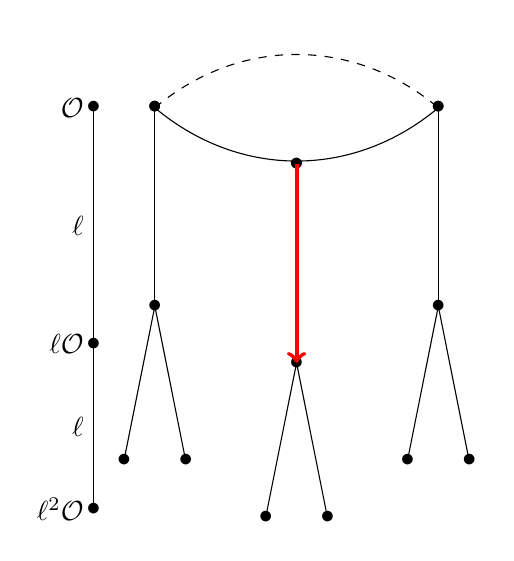
\begin{tikzpicture}[scale=0.60]
\coordinate (A) at (0,1.5);
\coordinate (AB) at (1,1.5);
%\coordinate (AZ) at (-1.5,1.5);	
\coordinate (B) at (0,5);
\coordinate (BB) at (1,5);
%\coordinate (BZ) at (-1.5,5.2);
%\coordinate (BZ2) at (-1.5,4.8);
\coordinate (C) at (0,10);
\coordinate (CB) at (1,10);
%\coordinate (CZ) at (-1.5,10);
\draw (A) node[left]{$\ell^2 \mathcal{O}$} node{$\bullet$};
\draw (B) node[left]{$\ell \mathcal{O}$} node{$\bullet$};
\draw (C) node[left]{$\mathcal{O}$} node{$\bullet$};
\draw (A)--(B)node[midway,left] {$\ell$};
\draw (B)--(C) node[midway,left] {$\ell$};
%\draw (CZ)--(BZ)[dashed]  node[midway,left] {$\ell$};
%\draw (BZ2)--(AZ)[dashed]  node[midway,left] {$\ell$};
\begin{scope}[yshift=10cm]
	\begin{scope}[xshift=4.3cm]
		\node (A) at (-3,0) {$\bullet$};
		\node (B) at (3,0) {$\bullet$};
		\node (C) at (270:1.2) {$\bullet$};
		\node (D) at (90:1.5) {};
		%\draw[-] (A.center) to[bend right=25] (C.center);
		\draw[-,dashed] (A.center) to[bend left=40] (B.center);
		%\draw[-] (B.center) to[bend left=25] (C.center);
		%\draw[-,dashed] (B.center) to[bend right] (D.center);
		\draw[-] (A.center) to[bend right=40] (B.center);
			\begin{scope}[xshift=-3cm]
			\coordinate (A) at (0,0);
			\coordinate (C) at (270:4.2);
			\coordinate (CA) at (265:7.5);
			\coordinate (CB) at (275:7.5);
			\draw (C)--(CA);
			\draw (C)--(CB);
			\draw (CA) node{$\bullet$};
			\draw (CB) node{$\bullet$};
			\draw (A) node{$\bullet$};
			\draw (C) node{$\bullet$};
			\draw (A)--(C);
			\end{scope}
			\begin{scope}[xshift=3cm]
			\coordinate (A) at (0,0);
			\coordinate (C) at (270:4.2);
			\coordinate (CA) at (265:7.5);
			\coordinate (CB) at (275:7.5);
			\draw (C)--(CA);
			\draw (C)--(CB);
			\draw (CA) node{$\bullet$};
			\draw (CB) node{$\bullet$};
			\draw (A) node{$\bullet$};
			\draw (C) node{$\bullet$};
			\draw (A)--(C);
			\end{scope}
			\begin{scope}[yshift=-1.2cm]
			\coordinate (A) at (0,0);
			\coordinate (C) at (270:4.2);
			\coordinate (CA) at (265:7.5);
			\coordinate (CB) at (275:7.5);
			\draw (C)--(CA);
			\draw (C)--(CB);
			\draw (CA) node{$\bullet$};
			\draw (CB) node{$\bullet$};
			\draw (A) node{$\bullet$};
			\draw (C) node{$\bullet$};
			\draw[line width=1.5pt,red,->] (A)--(C);
			\end{scope}
	\end{scope}
\end{scope}

%faire des fleches courbees avec les indices \ell et \ell^2


\end{tikzpicture}
\end{center}		
\end{figure}}

\only<2-2>{
\begin{figure}
\begin{center}

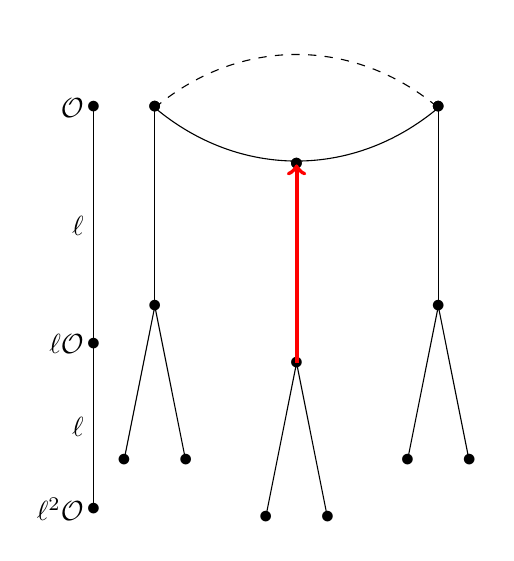
\begin{tikzpicture}[scale=0.60]
\coordinate (A) at (0,1.5);
\coordinate (AB) at (1,1.5);
%\coordinate (AZ) at (-1.5,1.5);	
\coordinate (B) at (0,5);
\coordinate (BB) at (1,5);
%\coordinate (BZ) at (-1.5,5.2);
%\coordinate (BZ2) at (-1.5,4.8);
\coordinate (C) at (0,10);
\coordinate (CB) at (1,10);
%\coordinate (CZ) at (-1.5,10);
\draw (A) node[left]{$\ell^2 \mathcal{O}$} node{$\bullet$};
\draw (B) node[left]{$\ell \mathcal{O}$} node{$\bullet$};
\draw (C) node[left]{$\mathcal{O}$} node{$\bullet$};
\draw (A)--(B)node[midway,left] {$\ell$};
\draw (B)--(C) node[midway,left] {$\ell$};
%\draw (CZ)--(BZ)[dashed]  node[midway,left] {$\ell$};
%\draw (BZ2)--(AZ)[dashed]  node[midway,left] {$\ell$};
\begin{scope}[yshift=10cm]
	\begin{scope}[xshift=4.3cm]
		\node (A) at (-3,0) {$\bullet$};
		\node (B) at (3,0) {$\bullet$};
		\node (C) at (270:1.2) {$\bullet$};
		\node (D) at (90:1.5) {};
		%\draw[-] (A.center) to[bend right=25] (C.center);
		\draw[-,dashed] (A.center) to[bend left=40] (B.center);
		%\draw[-] (B.center) to[bend left=25] (C.center);
		%\draw[-,dashed] (B.center) to[bend right] (D.center);
		\draw[-] (A.center) to[bend right=40] (B.center);
			\begin{scope}[xshift=-3cm]
			\coordinate (A) at (0,0);
			\coordinate (C) at (270:4.2);
			\coordinate (CA) at (265:7.5);
			\coordinate (CB) at (275:7.5);
			\draw (C)--(CA);
			\draw (C)--(CB);
			\draw (CA) node{$\bullet$};
			\draw (CB) node{$\bullet$};
			\draw (A) node{$\bullet$};
			\draw (C) node{$\bullet$};
			\draw (A)--(C);
			\end{scope}
			\begin{scope}[xshift=3cm]
			\coordinate (A) at (0,0);
			\coordinate (C) at (270:4.2);
			\coordinate (CA) at (265:7.5);
			\coordinate (CB) at (275:7.5);
			\draw (C)--(CA);
			\draw (C)--(CB);
			\draw (CA) node{$\bullet$};
			\draw (CB) node{$\bullet$};
			\draw (A) node{$\bullet$};
			\draw (C) node{$\bullet$};
			\draw (A)--(C);
			\end{scope}
			\begin{scope}[yshift=-1.2cm]
			\coordinate (A) at (0,0);
			\coordinate (C) at (270:4.2);
			\coordinate (CA) at (265:7.5);
			\coordinate (CB) at (275:7.5);
			\draw (C)--(CA);
			\draw (C)--(CB);
			\draw (CA) node{$\bullet$};
			\draw (CB) node{$\bullet$};
			\draw (A) node{$\bullet$};
			\draw (C) node{$\bullet$};
			\draw[line width=1.5pt,red,<-] (A)--(C);
			\end{scope}
	\end{scope}
\end{scope}

%faire des fleches courbees avec les indices \ell et \ell^2


\end{tikzpicture}
\end{center}		
\end{figure}}

\only<3-3>{
\begin{figure}
\begin{center}

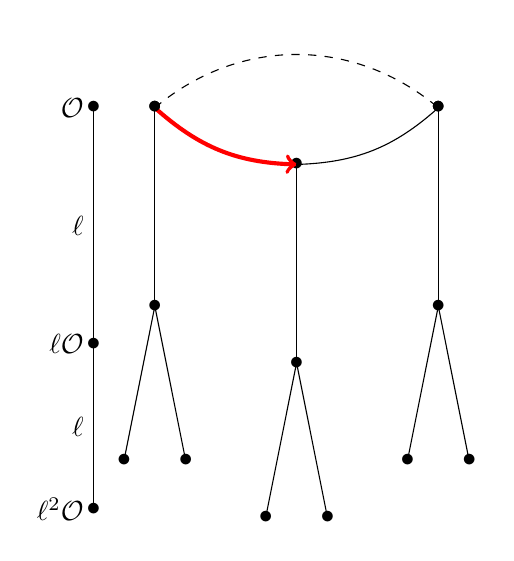
\begin{tikzpicture}[scale=0.60]
\coordinate (A) at (0,1.5);
\coordinate (AB) at (1,1.5);
%\coordinate (AZ) at (-1.5,1.5);	
\coordinate (B) at (0,5);
\coordinate (BB) at (1,5);
%\coordinate (BZ) at (-1.5,5.2);
%\coordinate (BZ2) at (-1.5,4.8);
\coordinate (C) at (0,10);
\coordinate (CB) at (1,10);
%\coordinate (CZ) at (-1.5,10);
\draw (A) node[left]{$\ell^2 \mathcal{O}$} node{$\bullet$};
\draw (B) node[left]{$\ell \mathcal{O}$} node{$\bullet$};
\draw (C) node[left]{$\mathcal{O}$} node{$\bullet$};
\draw (A)--(B)node[midway,left] {$\ell$};
\draw (B)--(C) node[midway,left] {$\ell$};
%\draw (CZ)--(BZ)[dashed]  node[midway,left] {$\ell$};
%\draw (BZ2)--(AZ)[dashed]  node[midway,left] {$\ell$};
\begin{scope}[yshift=10cm]
	\begin{scope}[xshift=4.3cm]
		\node (A) at (-3,0) {$\bullet$};
		\node (B) at (3,0) {$\bullet$};
		\node (C) at (270:1.2) {$\bullet$};
		\node (D) at (90:1.5) {};
		%\draw[-] (A.center) to[bend right=25] (C.center);
		\draw[-,dashed] (A.center) to[bend left=40] (B.center);
		%\draw[-] (B.center) to[bend left=25] (C.center);
		%\draw[-,dashed] (B.center) to[bend right] (D.center);
		\draw[-] (C.center) to[bend right=20] (B.center);
		\draw[line width=1.5pt,red,->] (A.center) to[bend right=20] (C.center);
			\begin{scope}[xshift=-3cm]
			\coordinate (A) at (0,0);
			\coordinate (C) at (270:4.2);
			\coordinate (CA) at (265:7.5);
			\coordinate (CB) at (275:7.5);
			\draw (C)--(CA);
			\draw (C)--(CB);
			\draw (CA) node{$\bullet$};
			\draw (CB) node{$\bullet$};
			\draw (A) node{$\bullet$};
			\draw (C) node{$\bullet$};
			\draw (A)--(C);
			\end{scope}
			\begin{scope}[xshift=3cm]
			\coordinate (A) at (0,0);
			\coordinate (C) at (270:4.2);
			\coordinate (CA) at (265:7.5);
			\coordinate (CB) at (275:7.5);
			\draw (C)--(CA);
			\draw (C)--(CB);
			\draw (CA) node{$\bullet$};
			\draw (CB) node{$\bullet$};
			\draw (A) node{$\bullet$};
			\draw (C) node{$\bullet$};
			\draw (A)--(C);
			\end{scope}
			\begin{scope}[yshift=-1.2cm]
			\coordinate (A) at (0,0);
			\coordinate (C) at (270:4.2);
			\coordinate (CA) at (265:7.5);
			\coordinate (CB) at (275:7.5);
			\draw (C)--(CA);
			\draw (C)--(CB);
			\draw (CA) node{$\bullet$};
			\draw (CB) node{$\bullet$};
			%\draw (A) node{$\bullet$};
			\draw (C) node{$\bullet$};
			\draw (A)--(C);
			\end{scope}
	\end{scope}
\end{scope}

%faire des fleches courbees avec les indices \ell et \ell^2


\end{tikzpicture}
\end{center}		
\end{figure}}


\end{column}
\begin{column}[left]{4cm}
\begin{lem}[Kohel 1996]
$E$ and $E'$ two elliptic curves defined over $\mathbb{F}_q$, $\phi :E \rightarrow E'$ an $\ell$-isogeny. Then
\begin{enumerate}
\item  $\ell=[\mathcal{O} : \mathcal{O}']$ we say then that $\phi$ is a 
\only<2-2> {descending isogeny,}
\only<3-3> {descending isogeny,}
\only<1-1>{$\textbf{descending}$ isogeny,}

\pause
\item $\ell=[\mathcal{O}':\mathcal{O}]$ we say then that $\phi$ is an \only<2-2> {$\textbf{ascending}$}
\only<3-3> {ascending} isogeny,
\pause 
\item $\mathcal{O}=\mathcal{O}'$ we say then that $\phi$ is an $\textbf{horizontal}$ isogeny.
\end{enumerate}
\end{lem}
%\begin{defi}
%The index $f=[\mathcal{O}_K : \mathcal{O}]$ is called the conductor of $\mathcal{O}$.
%\end{defi}
\end{column}

\end{columns}
\end{frame}

\begin{frame}
\section{Volcano of $\ell$-isogeny and Frobenius endomorphism}
\begin{figure}[h]
		\begin{center}
        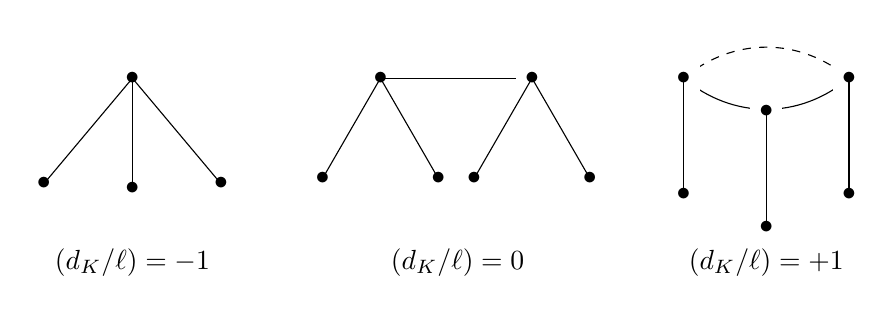
\begin{tikzpicture}[scale=0.35]
        \coordinate (A) at (0,0);
		\coordinate (B) at (230:5);
		\coordinate (C) at (270:4);
		\coordinate (D) at (310:5);
		\draw (A) node{$\bullet$};
		\draw (B) node[fill=white]{$\bullet$};
		\draw (C) node[fill=white]{$\bullet$};
		\draw (D) node[fill=white]{$\bullet$};
		\node at (0,-6.7) {$(d_K/\ell) = -1$};
		\draw (A)--(B);
		\draw (A)--(C);
		\draw (A)--(D);		
		\begin{scope}[xshift=9cm]
		\coordinate (A) at (0,0);
		\coordinate (B) at (5.5,0);
		\coordinate (C) at (240:4.2);
		\coordinate (D) at (300:4.2);
		\draw (A) node[fill=white]{$\bullet$};
		\draw (B) node[fill=white]{$\bullet$};
		\draw (C) node[fill=white]{$\bullet$};
		\draw (D) node[fill=white]{$\bullet$};
		\node at (2.8,-6.7) {$(d_K/\ell) = 0$};
		\draw (A)--(B);
		\draw (A)--(C);
		\draw (A)--(D);
		\end{scope}
		
		\begin{scope}[xshift=14.5cm]
		\coordinate (A) at (0,0);
		\coordinate (C) at (240:4.2);
		\coordinate (D) at (300:4.2);
		\draw (A) node[fill=white]{$\bullet$};
		\draw (C) node[fill=white]{$\bullet$};
		\draw (D) node[fill=white]{$\bullet$};
		\draw (A)--(C);
		\draw (A)--(D);
		\end{scope}
		
		\begin{scope}[xshift=23cm]
		\node (A) at (-3,0) {$\bullet$};
		\node (B) at (3,0) {$\bullet$};
		\node (C) at (270:1.2) {$\bullet$};
		\node (D) at (90:1.5) {};
		\node at (0,-6.7) {$(d_K/\ell) = +1$};
		%\draw[-] (A.center) to[bend right=25] (C.center);
		\draw[-,dashed] (A.center) to[bend left=40] (B.center);
		%\draw[-] (B.center) to[bend left=25] (C.center);
		%\draw[-,dashed] (B.center) to[bend right] (D.center);
		\draw[-] (A.center) to[bend right=40] (B.center);
			\begin{scope}[xshift=-3cm]
			\coordinate (A) at (0,0);
			\coordinate (C) at (270:4.2);
			\draw (A) node[fill=white]{$\bullet$};
			\draw (C) node[fill=white]{$\bullet$};
			\draw (A)--(C);
			\end{scope}
			\begin{scope}[xshift=3cm]
			\coordinate (A) at (0,0);
			\coordinate (C) at (270:4.2);
			\draw (A) node[fill=white]{$\bullet$};
			\draw (C) node[fill=white]{$\bullet$};
			\draw (A)--(C);
			\end{scope}
			\begin{scope}[yshift=-1.2cm]
			\coordinate (A) at (0,0);
			\coordinate (C) at (270:4.2);
			\draw (A) node[fill=white]{$\bullet$};
			\draw (C) node[fill=white]{$\bullet$};
			\draw (A)--(C);
			\end{scope}
		\end{scope}
		\end{tikzpicture}
		%\end{center}
		\caption{The three shapes of volcanoes of $2$-isogenies }
		
		\end{center} 
		\end{figure}
In the rest of this talk we consider only volcanoes with cyclic crater.
%\begin{figure}[hbtp]
%\centering
%\includegraphics[scale=0.4]{Images/duo-volcan-wo-label.png}
%\caption{Volcano with one point on the crater, and two points}
%\end{figure}
\end{frame}

\begin{frame}
\frametitle{Motivation}
We focus on one specific subproblem in the Schoof-Elkies-Atkin point counting  algorithm:
\medskip
\orangebox{Explicit isogeny computation problem}
{
 Let $\mathbb{F}_q$ be a finite field of characteristic $p$. 
 Given $E$, $E'$   two $r$-isogenous elliptic curves defined over $\mathbb{F}_q$,
 compute an $r$-isogeny $\phi:E\to E'$.
}
\end{frame}

\begin{frame}
\frametitle{Previous work}

Let $q=p^n$

\begin{itemize}
\item{} [Elkies '92/'98],  [CCR '91], [BMSS '08] work only for $r \ll p$ using $\tilde{O}(r)$ operations in $\mathbb{F}_q$.
\item{} [Couveignes '94] $\tilde{O}(r^3)$
\item{} [Couveignes '96] works using $\tilde{O}(r^2)$ operations in $\mathbb{F}_q$, but has exponential complexity in $\log(p)$.
\item{} [Lercier '97] only $p=2$.
\item{} [LS '08] works for every $p$ using $\tilde{O}(r^2)$ operations in $\mathbb{F}_q$
\end{itemize}
\begin{itemize}

\item[$\rightarrow$] we focus on the medium characteristic case,

\item[$\rightarrow$] we want to modify Couveignes' algorithm to obtain an algorithm with complexity $\tilde{O}(r^2)$ but with no exponential dependency in $\log(p)$

\end{itemize}
\end{frame}


\begin{frame}
\frametitle{Couveignes algorithm (1996)}
\bluebox{Couveignes' algorithm}{ %\cite{DBLP:conf/ants/Couveignes96}}{
\begin{algorithmic}[1]
\REQUIRE $E, E'$ two $r$-isogenous curves on $\mathbb{F}_{p^n}$ 
\ENSURE $\phi: E \rightarrow E'$ of degree $r$
\end{algorithmic}}
Couveignes' algorithm:
\begin{enumerate}
\begin{enumerate}
\item Fix $k$ such that $p^k>4r$;
\item Compute generators $P$ of
  $E[p^k]$ and $P'$ of $E'[p^k]$;
\item\label{alg:ours:T} Compute the polynomial~$T=\prod(X-x_i)$ of degree $\frac{p^k-1}{2}$ with $x_i$
  $x$-coordinates of $\langle P\rangle$;

\item\label{alg:ours:for} For each $a \in \left( \mathbb{Z}/p^k\mathbb{Z}\right)^{\times}$:
 \begin{enumerate}
  \item\label{alg:ours:interp} compute the interpolation polynomial
    $L_{a}$ such that
    $L_{a} (x (u P)) = x(a\, u\,P' )$ for
    $u \in \mathbb{Z}/p^k \mathbb{Z}$;
  \item\label{alg:ours:cauchy} Use a  rational reconstruction  algorithm 
    to compute a rational
    fraction $F_{a}=L_{a}\bmod{T}$ of degrees~$(r, r-1)$;
  \item If $F_{a}$ defines an isogeny of degree $r$, return it and
    stop.
  \end{enumerate}
\end{enumerate}
\end{enumerate}
Complexity polynomial in $p$. \textbf{Goal:} replace $E[p^k]$ by \boldmath $E[\ell^k]$ \unboldmath for a small $\ell$.
\end{frame}

\begin{frame}

\frametitle{Computing isogenies}
\bluebox{}{
Our goal is to work with \boldmath $E[\ell^k]= \left(\mathbb{Z}/\ell^k \mathbb{Z} \right)^2$ \unboldmath 
%Our goal is to work with \textcolor{red}{$E[\ell^k]= \left(\mathbb{Z}/\ell^k \mathbb{Z} \right)^2$}  
instead of $E[p^k]$ to remove the dependency in the characteristic $p$ of the finite field.
\begin{itemize}
\pause
%\item[$\Rightarrow$] main drawback: $E[\ell^{\frac{k}{2}}]=\left(\mathbb{Z}/\ell^{\frac{k}{2}} \mathbb{Z} \right)^2$ thus for two basis $\langle P,Q \rangle=E[\ell^{\frac{k}{2}}]$, $\langle P',Q' \rangle=E'[\ell^{\frac{k}{2}}]$ we have to test $O(\ell^{\frac{4k}{2}})=O(r^2)$ mapping candidates before finding the good one for the interpolation.
\item $E[p^k]=\left(\mathbb{Z}/p^{k} \mathbb{Z} \right) \quad \quad \quad \quad$  with $p^{k}>4r$
\item $E[\ell^k]=\left(\mathbb{Z}/\ell^{k} \mathbb{Z} \right) \times \left(\mathbb{Z}/\ell^{k} \mathbb{Z} \right)$ with $\ell^{2k}>4r$

\pause

\end{itemize}}
Therefore we study the $\ell$-torsion and the action of the Frobenius endomorphism on it.
\end{frame}

\begin{frame}
%Diapo sur le Frobenius....
%We want to study the action of the Frobenius on the $\ell$ torsion:

We denote by $T_{\ell}(E)$ the Tate module on the elliptic curve $E$, we study the action of the Frobenius endormorphism $\pi$ on it.
%\begin{prop}
%For $E$ an ordinary elliptic curve defined over $\mathbb{F}_q$ of characteristic $p$ the Tate module has the following structure for $\ell \neq p$:
%\[ T_{\ell}(E) \cong \mathbb{Z}_{\ell} \times \mathbb{Z}_{\ell} \]
%\end{prop}
\orangebox{Elkies prime}{
As we work on cyclic craters, the Frobenius endomorphism has two distinct eigenvalues denoted $\color{red}{\lambda}$, $\color{blue}{\mu}$.
}
\pause
Ou goal is to specify a part of the Tate module $T_{\ell}(E)$:
\[
\color{red}T_{\lambda}(E) \color{black} \oplus \color{blue} T_{\mu}(E) \color{black} \bmod \ell^k
\]
with $\color{red}{T_{\lambda}(E)}, \color{blue}{T_{\mu}(E)}$ eigenvectors for the eigenvalues $\color{red}{ \lambda}$, $\color{blue}{ \mu}$.
%\begin{rem}
%\begin{itemize}
%\item Then the action of the Frobenius endomorphism on $T_{\ell}(E)$, which we write~$\pi|T_{\ell}(E)$, has two distinct eigenvalues: $\lambda, \mu $
%
%%Moreover the depth of the volcano of $\mathbb{F}_q$-rational $\ell$-isogenies is~$h = v_\ell(\lambda-\mu)$.
%\item We denote by $h$ the height of the volcano of $\mathbb{F}_q$-rational $\ell$-isogenies.
%\end{itemize}
%\end{rem}


\end{frame}




%\begin{frame}
%
%\begin{prop} \label{prop:diagonal-horizontal}
%Let~$E$ be a curve lying on the crater and~$P$ be a point of~$E[\ell^k]$.
%Then $ P$~is horizontal if and only if its preimages by multiplication by 
%$\ell^h$ are eigenvectors for~$\pi$.
%Let $P_0$ be such a preimage if $\pi(P_0) = \lambda P_0$ then we say that $P$~has direction~$\lambda$.
%\end{prop}
%
%Thus we will work only with curves for which we have $\pi|T_\ell(E)$ conjugate, over~$\mathbb{Z}_\ell$ to a diagonal matrix.
%
%\end{frame}


%\begin{frame}
%
%
%%Then the point $P=(36,96)$ computed as described earlier verifies that $\pi(P)=\lambda P$. Since $P$ is of order $2^3$ then we have $2^{2}P=(42,0)$ which is horizontal, the $2$-isogeny generated by $2^{2}P$ goes to another curve on the crater: $E2$. The points $2P$ is not necessarily horizontal. 
%\end{exe}
%\end{frame}

\begin{frame}
\begin{columns}
\begin{column}[l]{4cm}
\begin{exe}[Volcano with height=0]
When we got a diagonalisation of the Frobenius endomorphism $\pi$:
\only<1-1>{
\[
\left( \begin{matrix}
\lambda & 0 \\
0 & \mu 
\end{matrix} \right) \bmod \textit{\boldmath  $\ell$ \unboldmath } 
\]
then we have determined a part of $T_{\ell}(E)$:
\[
\color{red} T_{\lambda}(E) \color{black} \oplus \color{blue} T_{\mu}(E) \color{black} \bmod \ell
\]
}
\only<2-2>{
\[
\left( \begin{matrix}
\lambda & 0 \\
0 & \mu 
\end{matrix} \right) \bmod \textit{\boldmath  $\ell^2$ \unboldmath } 
\]
then we have determined a part of $T_{\ell}(E)$:
\[
\color{red} T_{\lambda}(E) \color{black} \oplus \color{blue} T_{\mu}(E) \color{black} \bmod \ell^2
\]
}

\only<3-3>{
\[
\left( \begin{matrix}
\lambda & 0 \\
0 & \mu 
\end{matrix} \right) \bmod \textit{\boldmath  $\ell^3$ \unboldmath } 
\]
then we have determined a part of $T_{\ell}(E)$:
\[
\color{red} T_{\lambda}(E) \color{black} \oplus \color{blue} T_{\mu}(E) \color{black} \bmod \ell^3
\]
}
\end{exe}

%CITER François et Jean Marc ici...
\end{column}
\begin{column}[r]{6cm}
\only<1-1>{
\begin{figure}[h]
	\begin{center}
	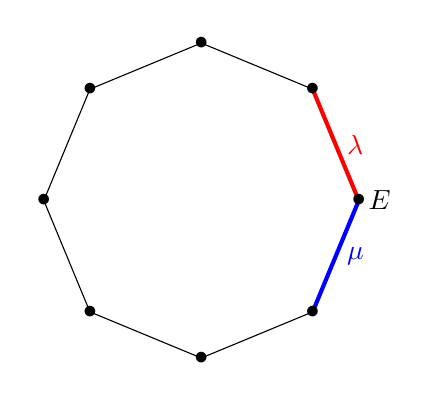
\begin{tikzpicture}[scale=0.4]
	\coordinate (A) at (0:5);
	\coordinate (B) at (45:5);
	\coordinate (C) at (90:5);
	\coordinate (D) at (135:5);
	\coordinate (E) at (180:5);
	\coordinate (F) at (225:5);
	\coordinate (G) at (270:5);
	\coordinate (H) at (315:5);
	\draw (A)--(B)--(C)--(D)--(E)--(F)--(G)--(H)--(A);		
	\draw[line width=1.5pt,red] (A)--(B) node[midway,right]{$\color{red} \lambda$};
	\draw[line width=1.5pt,blue] (A)--(H) node[midway,right]{$\color{blue} \mu$};
	
	
	
	\draw (A) node{$\bullet$};
	\draw (A) node[right]{$E$};
	\draw (B) node{$\bullet$};
	\draw (C) node{$\bullet$};
	\draw (D) node{$\bullet$};
	\draw (E) node{$\bullet$};
	\draw (F) node{$\bullet$};
	\draw (G) node{$\bullet$};
	\draw (H) node{$\bullet$};
	\end{tikzpicture}	
	\end{center}
\end{figure}}
\only<2-2>{
\begin{figure}[h]
	\begin{center}
	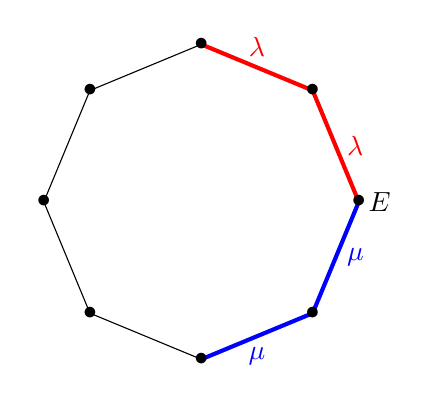
\begin{tikzpicture}[scale=0.4]
	\coordinate (A) at (0:5);
	\coordinate (B) at (45:5);
	\coordinate (C) at (90:5);
	\coordinate (D) at (135:5);
	\coordinate (E) at (180:5);
	\coordinate (F) at (225:5);
	\coordinate (G) at (270:5);
	\coordinate (H) at (315:5);
	\draw (A)--(B)--(C)--(D)--(E)--(F)--(G)--(H)--(A);		
	\draw[line width=1.5pt,red] (A)--(B) node[midway,right]{$\color{red} \lambda$};
	\draw[line width=1.5pt,blue] (A)--(H) node[midway,right]{$\color{blue} \mu$};
	\draw[line width=1.5pt,red] (B)--(C) node[midway,above]{$\color{red} \lambda$};
	\draw[line width=1.5pt,blue] (H)--(G) node[midway,below]{$\color{blue} \mu$};
		
	\draw (A) node[right]{$E$};
	\draw (A) node{$\bullet$};
	\draw (B) node{$\bullet$};
	\draw (C) node{$\bullet$};
	\draw (D) node{$\bullet$};
	\draw (E) node{$\bullet$};
	\draw (F) node{$\bullet$};
	\draw (G) node{$\bullet$};
	\draw (H) node{$\bullet$};
	\end{tikzpicture}	
	\end{center}
\end{figure}}
\only<3-3>{
\begin{figure}[h]
	\begin{center}
	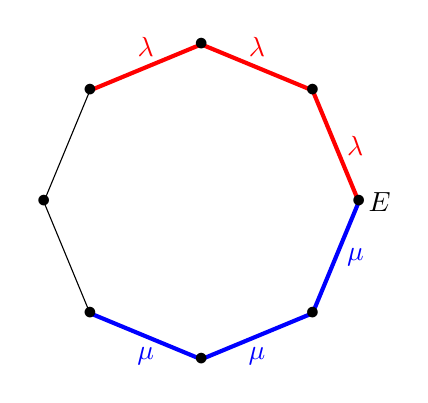
\begin{tikzpicture}[scale=0.4]
	\coordinate (A) at (0:5);
	\coordinate (B) at (45:5);
	\coordinate (C) at (90:5);
	\coordinate (D) at (135:5);
	\coordinate (E) at (180:5);
	\coordinate (F) at (225:5);
	\coordinate (G) at (270:5);
	\coordinate (H) at (315:5);
	\draw (A)--(B)--(C)--(D)--(E)--(F)--(G)--(H)--(A);		
	\draw[line width=1.5pt,red] (A)--(B) node[midway,right]{$\color{red} \lambda$};
	\draw[line width=1.5pt,blue] (A)--(H) node[midway,right]{$\color{blue} \mu$};
	\draw[line width=1.5pt,red] (B)--(C) node[midway,above]{$\color{red} \lambda$};
	\draw[line width=1.5pt,blue] (H)--(G) node[midway,below]{$\color{blue} \mu$};
	\draw[line width=1.5pt,red] (C)--(D) node[midway,above]{$\color{red} \lambda$};
	\draw[line width=1.5pt,blue] (G)--(F) node[midway,below]{$\color{blue} \mu$};
		
	\draw (A) node[right]{$E$};
	\draw (A) node{$\bullet$};
	\draw (B) node{$\bullet$};
	\draw (C) node{$\bullet$};
	\draw (D) node{$\bullet$};
	\draw (E) node{$\bullet$};
	\draw (F) node{$\bullet$};
	\draw (G) node{$\bullet$};
	\draw (H) node{$\bullet$};
	\end{tikzpicture}	
	\end{center}
\end{figure}}
\end{column}
\end{columns}
\end{frame}

\begin{frame}

\begin{prop}\label{prop:matrice-Frobenius}
Let $E$ be a curve on a crater of an $\ell$-isogeny volcano.
%Then there exists a unique $a \in \{ 0,\ell, \dots, \ell^{h-1}  \}$
%such that $\pi|T_\ell(E)$~is conjugate, over~$\mathbb{Z}_\ell$,
%to the matrix $\left ( \begin{smallmatrix}\lambda & a\\ 0 & \mu
%\end{smallmatrix}\right )$.
% where $a ∈ ℤ$, $0 ≤ a ≤ ℓ^{h} - 1$,
Then the action of the Frobenius endomorphism $\pi$ on $T_\ell(E)$~is conjugate, over~$\mathbb{Z}_\ell$,
to the matrix \[\left ( \begin{matrix}\lambda & a\\ 0 & \mu \end{matrix}\right ) \]  with $a \in \{ 0,1,\ell, \dots, \ell^{h-1}  \}$ and $a = 0$ if~$E$ lies on the crater.

%Moreover $a = 0$ if~$E$ lies on the crater.
%and else $h - v_{\ell}(a)$~is the depth of~$E$ in the volcano.
\end{prop}

\begin{figure}
\begin{center}

\begin{tikzpicture}[scale=0.30]
\coordinate (A) at (0,1.5);
\coordinate (AB) at (1,1.5);
\coordinate (AZ) at (-1.5,1.5);	
\coordinate (B) at (0,5);
\coordinate (BB) at (1,5);
\coordinate (BZ) at (-1.5,5.2);
\coordinate (BZ2) at (-1.5,4.8);
\coordinate (C) at (0,10);
\coordinate (CB) at (1,10);
\coordinate (CZ) at (-1.5,10);
\draw (A) node[left]{$\color{cyan}\left( \begin{matrix}
\lambda & \ell^2 \\
0 & \mu
\end{matrix} \right) \color{black} $}; %node{$\bullet$};
\draw (B) node[left]{$\color{magenta} \left( \begin{matrix}
\lambda & \ell \\
0 & \mu
\end{matrix} \right) \color{black} $}; %node{$\bullet$};
\draw (C) node[left]{$\color{green} \left( \begin{matrix}
\lambda & 0 \\
0 & \mu
\end{matrix} \right) \color{black} $}; %node{$\bullet$};
%\draw (A)--(B);
%\draw (B)--(C);
%\draw (CZ)--(BZ)[dashed]  node[midway,left] {$\ell$};
%\draw (BZ2)--(AZ)[dashed]  node[midway,left] {$\ell$};
\begin{scope}[yshift=10cm]
	\begin{scope}[xshift=4.3cm]
		\node (A) at (-3,0) {$ \color{green} \bullet $};
		\node (B) at (3,0) {$  \color{green} \bullet$};
		\node (C) at (270:1.2) {$\color{green} \bullet \color{black}$};
		\node (D) at (90:1.5) {};
		%\draw[-] (A.center) to[bend right=25] (C.center);
		\draw[-,dashed] (A.center) to[bend left=40] (B.center);
		%\draw[-] (B.center) to[bend left=25] (C.center);
		%\draw[-,dashed] (B.center) to[bend right] (D.center);
		\draw[-] (A.center) to[bend right=40] (B.center);
		\draw (A) node{$ \color{green} \bullet $};
		\draw (B) node{$ \color{green} \bullet $};
		\draw (C) node{$ \color{green} \bullet $};
		%\draw[line width=2.5pt,red,->] (A.center) to[bend right=20] (C.center);
			\begin{scope}[xshift=-3cm]
			\coordinate (A) at (0,0);
			\coordinate (C) at (270:4.2);
			\coordinate (CA) at (265:7.5);
			\coordinate (CB) at (275:7.5);
			\draw (C)--(CA);
			\draw (C)--(CB);
			\draw (A)--(C);
			\draw (CA) node{$\color{cyan} \bullet$};
			\draw (CB) node{$\color{cyan} \bullet$};
			\draw (A) node{$ \color{green} \bullet \color{black}$};
			\draw (C) node{$ \color{magenta} \bullet \color{bullet}$};
			\end{scope}
			\begin{scope}[xshift=3cm]
			\coordinate (A) at (0,0);
			\coordinate (C) at (270:4.2);
			\coordinate (CA) at (265:7.5);
			\coordinate (CB) at (275:7.5);
			\draw (C)--(CA);
			\draw (C)--(CB);
			\draw (A)--(C);
			\draw (CA) node{$\color{cyan} \bullet$};
			\draw (CB) node{$\color{cyan}\bullet$};
			\draw (A) node{$\color{green} \bullet$};
			\draw (C) node{$\color{magenta} \bullet$};
			\end{scope}
			\begin{scope}[yshift=-1.2cm]
			\coordinate (A) at (0,0);
			\coordinate (C) at (270:4.2);
			\coordinate (CA) at (265:7.5);
			\coordinate (CB) at (275:7.5);
			\draw (C)--(CA);
			\draw (C)--(CB);
			\draw (A)--(C);
			\draw (CA) node{$\color{cyan} \bullet$};
			\draw (CB) node{$\color{cyan} \bullet$};
			%\draw (A) node{$\bullet$};
			\draw (C) node{$\color{magenta} \bullet$};
			\draw (A) node{$\color{green} \bullet$};
			
			
			%(C) node[left]{$\mathcal{O}$} node{$\bullet$};			
			
			\end{scope}
			\coordinate (F) at (5,0);
			\coordinate (G) at (5,-7);
			\draw[dashed,<-] (F)--(G) node[midway,right]{$h$};
	\end{scope}
\end{scope}

%faire des fleches courbees avec les indices \ell et \ell^2


\end{tikzpicture}
\end{center}
\end{figure}
\end{frame}

\begin{frame}
\begin{columns}
\begin{column}[l]{5cm}
\orangebox{Volcano with height $h=0$}{
When we have partially diagonalized the Frobenius endormorphism on the Tate Module $T_{\ell}(E)$:
\[
\left( \begin{matrix}
\lambda & 0 \\
0 & \mu 
\end{matrix} \right) \bmod \textit{\boldmath  $\ell^3$ \unboldmath } 
\]
We get:
\begin{figure}[h]
	\begin{center}
	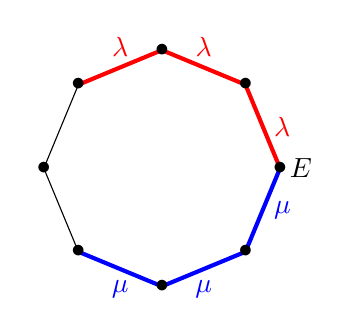
\begin{tikzpicture}[scale=0.3]
	\coordinate (A) at (0:5);
	\coordinate (B) at (45:5);
	\coordinate (C) at (90:5);
	\coordinate (D) at (135:5);
	\coordinate (E) at (180:5);
	\coordinate (F) at (225:5);
	\coordinate (G) at (270:5);
	\coordinate (H) at (315:5);
	\draw (A)--(B)--(C)--(D)--(E)--(F)--(G)--(H)--(A);		
	\draw[line width=1.5pt,red] (A)--(B) node[midway,right]{$\color{red} \lambda$};
	\draw[line width=1.5pt,blue] (A)--(H) node[midway,right]{$\color{blue} \mu$};
	\draw[line width=1.5pt,red] (B)--(C) node[midway,above]{$\color{red} \lambda$};
	\draw[line width=1.5pt,blue] (H)--(G) node[midway,below]{$\color{blue} \mu$};
	\draw[line width=1.5pt,red] (C)--(D) node[midway,above]{$\color{red} \lambda$};
	\draw[line width=1.5pt,blue] (G)--(F) node[midway,below]{$\color{blue} \mu$};
		
	\draw (A) node[right]{$E$};
	\draw (A) node{$\bullet$};
	\draw (B) node{$\bullet$};
	\draw (C) node{$\bullet$};
	\draw (D) node{$\bullet$};
	\draw (E) node{$\bullet$};
	\draw (F) node{$\bullet$};
	\draw (G) node{$\bullet$};
	\draw (H) node{$\bullet$};
	\end{tikzpicture}	
	\end{center}
\end{figure}
}
\end{column}
\begin{column}[r]{5cm}
\orangebox{Volcano with height $h=2$}{
When we have partially diagonalized the Frobenius endormorphism on the Tate Module $T_{\ell}(E_0)$:
\[
\left( \begin{matrix}
\lambda & 0 \\
0 & \mu 
\end{matrix} \right) \bmod \textit{\boldmath  $\ell^3$ \unboldmath } 
\]
\begin{figure}[h]
		\begin{center}
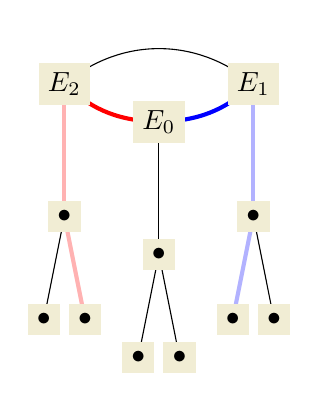
\begin{tikzpicture}[scale=0.40]
\begin{scope}[yshift=10cm]
	\begin{scope}[xshift=4.3cm]
		\node (A) at (-3,0) {$\bullet$};
		\node (B) at (3,0) {$\bullet$};
		\node (C) at (270:1.2) {$\bullet$};
		\node (D) at (90:1.5) {};
		%\draw[-] (A.center) to[bend right=25] (C.center);
		\draw[-] (A.center) to[bend left=40] (B.center);
		%\draw[-] (B.center) to[bend left=25] (C.center);
		%\draw[-,dashed] (B.center) to[bend right] (D.center);
		\draw[line width=1.5pt,blue,->] (C.center) to[bend right=20] (B.center);
		\draw [line width=1.5pt,red,<-] (A.center) to[bend right=20] (C.center);
			\begin{scope}[xshift=-3cm]
			\coordinate (A) at (0,0);
			\coordinate (C) at (270:4.2);
			\coordinate (CA) at (265:7.5);
			\coordinate (CB) at (275:7.5);
			\draw (C)--(CA);
			\draw [line width=1.5pt,color=red!30,->] (C)--(CB);
			\draw [line width=1.5pt,color=red!30,->] (A)--(C);
%			\draw (A) node[fill=white]{$30$};
%			\draw (C) node[fill=white]{$98$};
%			\draw (CA) node[fill=white]{$22$};
%			\draw (CB) node[fill=white]{$74$};
			\draw (A) node[fill=pacificcream]{$E_2$};
			\draw (C) node[fill=pacificcream]{$\bullet$};
			\draw (CA) node[fill=pacificcream]{$\bullet$};
			\draw (CB) node[fill=pacificcream]{$\bullet$};
			\end{scope}
			\begin{scope}[xshift=3cm]
			\coordinate (A) at (0,0);
			\coordinate (C) at (270:4.2);
			\coordinate (CA) at (265:7.5);
			\coordinate (CB) at (275:7.5);
			\draw [line width=1.5pt,color=blue!30,->] (C)--(CA);
			\draw (C)--(CB);
			\draw [line width=1.5pt,color=blue!30,->] (A)--(C);
%			\draw (A) node[fill=white]{$65$};
%			\draw (C) node[fill=white]{$60$};
%			\draw (CA) node[fill=white]{$39$};
%			\draw (CB) node[fill=white]{$62$};
			\draw (A) node[fill=pacificcream]{$E_1$};
			\draw (C) node[fill=pacificcream]{$\bullet$};
			\draw (CA) node[fill=pacificcream]{$\bullet$};
			\draw (CB) node[fill=pacificcream]{$\bullet$};
			\end{scope}
			\begin{scope}[yshift=-1.2cm]
			\coordinate (A) at (0,0);
			\coordinate (C) at (270:4.2);
			\coordinate (CA) at (265:7.5);
			\coordinate (CB) at (275:7.5);
			\draw (C)--(CA);
			\draw (C)--(CB);
			\draw (A)--(C);
%			\draw (A) node[fill=white]{$28$};
%			\draw (C) node[fill=white]{$27$};
%			\draw (CA) node[fill=white]{$45$};
%			\draw (CB) node[fill=white]{$68$};
			\draw (A) node[fill=pacificcream]{$E_0$};
			\draw (C) node[fill=pacificcream]{$\bullet$};
			\draw (CA) node[fill=pacificcream]{$\bullet$};
			\draw (CB) node[fill=pacificcream]{$\bullet$};
			\end{scope}
	\end{scope}
\end{scope}
\end{tikzpicture}
		%\end{center}
		%\caption{Volcano of $2$-isogenies with height $h=2$}
		
		\end{center} 
		\end{figure}
}
\end{column}
\end{columns}
\end{frame}

\begin{frame}
%Frame sur les bases horizontales, diagonales.
\begin{defi}[Horizontal and diagonal bases]
  Let~$E$ be a curve lying on the crater. We call a
  basis of~$E[\ell^k]$
\begin{itemize}
		  
 {\setlength\itemindent{25pt} \item[\emph{diagonal}] if $\pi$~is diagonal in it;}
  {\setlength\itemindent{25pt} \item[\emph{horizontal}] if both basis points generate the kernel of
  horizontal $\ell^k$-isogenies. }

\end{itemize}  
  Accordingly, we also call diagonal
  (resp. horizontal) the generators of a diagonal (resp. horizontal)
  basis.
\end{defi}

\orangebox{Fact}{Horizontal bases are diagonal bases.}
\end{frame}



\begin{frame}
\begin{columns}

\begin{column}[l]{4cm}
\begin{exe}[Volcano with height=2]
Let $E_0$ be the curve with $j$-invariant $28$ and defined on $\mathbb{F}_{101}$ by: 
\[y^2=x^3+85x+11\]
$P=(36,96)$ a point of order $8$ verifies that $\pi(P)=\lambda P$


\begin{itemize}\only<1-1>{
\item \boldmath $P$ \unboldmath is  \textbf{not horizontal},}
\only<2-3>{\item $P$ is not horizontal,}
\only<2-2>{\item \boldmath $2P$ \unboldmath is \textbf{not horizontal},}
\only<1,3>{\item $2P$ is not horizontal,}
\only<1-2>{\item $2^{2}P$ is horizontal.}
\only<3-3>{\item \boldmath $2^2P$ \unboldmath is \textbf{horizontal}.}
\end{itemize}


\end{exe}
\end{column}

\begin{column}[r]{7cm}
\begin{figure}[h]
		\begin{center}
		
\begin{tikzpicture}[scale=0.60]
\begin{scope}[yshift=10cm]
	\begin{scope}[xshift=4.3cm]
		\node (A) at (-3,0) {$\bullet$};
		\node (B) at (3,0) {$\bullet$};
		\node (C) at (270:1.2) {$\bullet$};
		\node (D) at (90:1.5) {};
		%\draw[-] (A.center) to[bend right=25] (C.center);
		\draw[-] (A.center) to[bend left=40] (B.center);
		%\draw[-] (B.center) to[bend left=25] (C.center);
		%\draw[-,dashed] (B.center) to[bend right] (D.center);
		\draw[-] (C.center) to[bend right=20] (B.center);
		\draw [line width=1.5pt,red,<-] (A.center) to[bend right=20] (C.center);
			\begin{scope}[xshift=-3cm]
			\coordinate (A) at (0,0);
			\coordinate (C) at (270:4.2);
			\coordinate (CA) at (265:7.5);
			\coordinate (CB) at (275:7.5);
			\draw (C)--(CA);
			\only<1-1>{
			\draw [line width=1.5pt,color=red!30,->] (C)--(CB);
			}
			\only<2-3>{
			\draw (C)--(CB);
			}
			\only<1-2>{
			\draw [line width=1.5pt,color=red!30,->] (A)--(C);
			}
			\only<3-3>{
			\draw (A)--(C);			
			}
%			\draw (A) node[fill=white]{$30$};
%			\draw (C) node[fill=white]{$98$};
%			\draw (CA) node[fill=white]{$22$};
%			\draw (CB) node[fill=white]{$74$};
			\draw (A) node[fill=white]{$E_2$};
			\draw (C) node[fill=white]{$\bullet$};
			\draw (CA) node[fill=white]{$\bullet$};
			\draw (CB) node[fill=white]{$\bullet$};
			\end{scope}
			\begin{scope}[xshift=3cm]
			\coordinate (A) at (0,0);
			\coordinate (C) at (270:4.2);
			\coordinate (CA) at (265:7.5);
			\coordinate (CB) at (275:7.5);
			\draw (C)--(CA);
			\draw (C)--(CB);
			\draw (A)--(C);
%			\draw (A) node[fill=white]{$65$};
%			\draw (C) node[fill=white]{$60$};
%			\draw (CA) node[fill=white]{$39$};
%			\draw (CB) node[fill=white]{$62$};
			\draw (A) node[fill=white]{$E_1$};
			\draw (C) node[fill=white]{$\bullet$};
			\draw (CA) node[fill=white]{$\bullet$};
			\draw (CB) node[fill=white]{$\bullet$};
			\end{scope}
			\begin{scope}[yshift=-1.2cm]
			\coordinate (A) at (0,0);
			\coordinate (C) at (270:4.2);
			\coordinate (CA) at (265:7.5);
			\coordinate (CB) at (275:7.5);
			\draw (C)--(CA);
			\draw (C)--(CB);
			\draw (A)--(C);
%			\draw (A) node[fill=white]{$28$};
%			\draw (C) node[fill=white]{$27$};
%			\draw (CA) node[fill=white]{$45$};
%			\draw (CB) node[fill=white]{$68$};
			\draw (A) node[fill=white]{$E_0$};
			\draw (C) node[fill=white]{$\bullet$};
			\draw (CA) node[fill=white]{$\bullet$};
			\draw (CB) node[fill=white]{$\bullet$};
			\end{scope}
	\end{scope}
\end{scope}
\end{tikzpicture}
		%\end{center}
		\caption{Volcano of $2$-isogenies on $\mathbb{F}_{101}$}
		
		\end{center} 
		\end{figure}
\end{column}
\end{columns}
\end{frame}

\begin{frame}
\begin{columns}

\begin{column}[l]{4cm}
\begin{exe}[Volcano with height=2]
When we got a diagonalisation of the Frobenius endomorphism $\pi$:
\[
\left( \begin{matrix}
\lambda & 0 \\
0 & \mu 
\end{matrix} \right) \bmod \textit{\boldmath  $\ell^3$ \unboldmath } 
\]
then we have determined a \emph{smaller} part of $T_{\ell}(E_0)$:
\[
\color{red}T_{\lambda} \color{black} \oplus \color{blue} T_{\mu} \color{black} \bmod \ell 
\]
\end{exe}
\end{column}

\begin{column}[r]{7cm}
\begin{figure}[h]
		\begin{center}
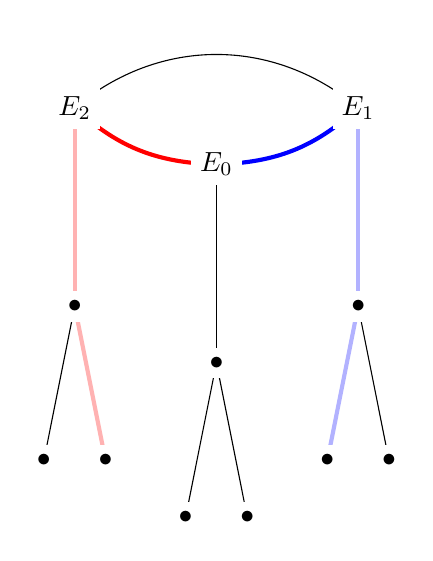
\begin{tikzpicture}[scale=0.60]
\begin{scope}[yshift=10cm]
	\begin{scope}[xshift=4.3cm]
		\node (A) at (-3,0) {$\bullet$};
		\node (B) at (3,0) {$\bullet$};
		\node (C) at (270:1.2) {$\bullet$};
		\node (D) at (90:1.5) {};
		%\draw[-] (A.center) to[bend right=25] (C.center);
		\draw[-] (A.center) to[bend left=40] (B.center);
		%\draw[-] (B.center) to[bend left=25] (C.center);
		%\draw[-,dashed] (B.center) to[bend right] (D.center);
		\draw[line width=1.5pt,blue,->] (C.center) to[bend right=20] (B.center);
		\draw [line width=1.5pt,red,<-] (A.center) to[bend right=20] (C.center);
			\begin{scope}[xshift=-3cm]
			\coordinate (A) at (0,0);
			\coordinate (C) at (270:4.2);
			\coordinate (CA) at (265:7.5);
			\coordinate (CB) at (275:7.5);
			\draw (C)--(CA);
			\draw [line width=1.5pt,color=red!30,->] (C)--(CB);
			\draw [line width=1.5pt,color=red!30,->] (A)--(C);
%			\draw (A) node[fill=white]{$30$};
%			\draw (C) node[fill=white]{$98$};
%			\draw (CA) node[fill=white]{$22$};
%			\draw (CB) node[fill=white]{$74$};
			\draw (A) node[fill=white]{$E_2$};
			\draw (C) node[fill=white]{$\bullet$};
			\draw (CA) node[fill=white]{$\bullet$};
			\draw (CB) node[fill=white]{$\bullet$};
			\end{scope}
			\begin{scope}[xshift=3cm]
			\coordinate (A) at (0,0);
			\coordinate (C) at (270:4.2);
			\coordinate (CA) at (265:7.5);
			\coordinate (CB) at (275:7.5);
			\draw [line width=1.5pt,color=blue!30,->] (C)--(CA);
			\draw (C)--(CB);
			\draw [line width=1.5pt,color=blue!30,->] (A)--(C);
%			\draw (A) node[fill=white]{$65$};
%			\draw (C) node[fill=white]{$60$};
%			\draw (CA) node[fill=white]{$39$};
%			\draw (CB) node[fill=white]{$62$};
			\draw (A) node[fill=white]{$E_1$};
			\draw (C) node[fill=white]{$\bullet$};
			\draw (CA) node[fill=white]{$\bullet$};
			\draw (CB) node[fill=white]{$\bullet$};
			\end{scope}
			\begin{scope}[yshift=-1.2cm]
			\coordinate (A) at (0,0);
			\coordinate (C) at (270:4.2);
			\coordinate (CA) at (265:7.5);
			\coordinate (CB) at (275:7.5);
			\draw (C)--(CA);
			\draw (C)--(CB);
			\draw (A)--(C);
%			\draw (A) node[fill=white]{$28$};
%			\draw (C) node[fill=white]{$27$};
%			\draw (CA) node[fill=white]{$45$};
%			\draw (CB) node[fill=white]{$68$};
			\draw (A) node[fill=white]{$E_0$};
			\draw (C) node[fill=white]{$\bullet$};
			\draw (CA) node[fill=white]{$\bullet$};
			\draw (CB) node[fill=white]{$\bullet$};
			\end{scope}
	\end{scope}
\end{scope}
\end{tikzpicture}
		%\end{center}
		\caption{Volcano of $2$-isogenies on $\mathbb{F}_{101}$}
		
		\end{center} 
		\end{figure}
\end{column}
\end{columns}
\end{frame}


\begin{frame}
\frametitle{How to build a horizontal basis from a diagonal basis}
\only<2-2>{
\transdissolve
}
\only<4-4>{
\transdissolve
}

\begin{columns}
\begin{column}[l]{5cm}
\orangebox{}{
On $E_0$ we have determined this part of $T_{\ell}(E_0)$:
\only<1-1>{
\[
\color{red}T_{\lambda} \color{black} \oplus \color{blue}T_{\mu} \color{black} \bmod \ell
\]}
\only<2-3>{
\[
\color{red}T_{\lambda} \color{black} \color{black} \bmod \ell^2
\]}
\only<4-4>{
\[
\color{red}T_{\lambda} \color{black} \color{black} \bmod \ell^3
\]}
}
\end{column}
\begin{column}[r]{7cm}
\begin{figure}
\begin{center}
\begin{tikzpicture}[scale=0.60]
\begin{scope}[yshift=10cm]
	\begin{scope}[xshift=4.3cm]
		\node (A) at (-3,0) {$\bullet$};
		\node (B) at (3,0) {$\bullet$};
		\node (C) at (270:1.2) {$\bullet$};
		\node (D) at (90:1.5) {};
		%\draw[-] (A.center) to[bend right=25] (C.center);
		\only<1-2>{		
		\draw[-] (A.center) to[bend left=40] (B.center);
		}
		\only<3-3>{
		\draw[line width=1.5pt,blue,->] (A.center) to[bend left=40] (B.center);
		\node (F) at (0,1.5) {$\color{blue} \mu$};		
		}
		\only<4-4>{
		\draw[line width=1.5pt,red,->] (A.center) to[bend left=40] (B.center);
		\node (F) at (0,1.5) {$\color{red} \lambda$};		
		}
		%\draw[-] (B.center) to[bend left=25] (C.center);
		%\draw[-,dashed] (B.center) to[bend right] (D.center);
		\only<1-1>{
		\draw[line width=1.5pt,blue,->] (C.center) to[bend right=20] (B.center); 
		\node (F) at (1.5,-0.5) {$\color{blue} \mu$};		
		}
		\only<2-4>{
		\draw[line width=1.5pt,red,<-] (C.center) to[bend right=20] (B.center); 
		\node (F) at (1.5,-0.5) {$\color{red} \lambda$};		
		}
		\draw [line width=1.5pt,red,<-] (A.center) to[bend right=20] (C.center);
		\node (E) at (-1.5,-0.5) {$\color{red} \lambda$};
		
			\begin{scope}[xshift=-3cm]
			\coordinate (A) at (0,0);
			\coordinate (C) at (270:4.2);
			\coordinate (CA) at (265:7.5);
			\coordinate (CB) at (275:7.5);
			\draw (C)--(CA);
			\only<1-1>{
			\draw [line width=1.5pt,color=red!30,->] (C)--(CB);}
			\only<2-4>{
			\draw (C)--(CB);}
			\only<1-3>{			
			\draw [line width=1.5pt,color=red!30,->] (A)--(C);}
			\only<4-4>{
			\draw (A)--(C);}
%			\draw (A) node[fill=white]{$30$};
%			\draw (C) node[fill=white]{$98$};
%			\draw (CA) node[fill=white]{$22$};
%			\draw (CB) node[fill=white]{$74$};
			\draw (A) node[fill=white]{$E_2$};
			\draw (C) node[fill=white]{$\bullet$};
			\draw (CA) node[fill=white]{$\bullet$};
			\draw (CB) node[fill=white]{$\bullet$};
			\end{scope}
			\begin{scope}[xshift=3cm]
			\coordinate (A) at (0,0);
			\coordinate (C) at (270:4.2);
			\coordinate (CA) at (265:7.5);
			\coordinate (CB) at (275:7.5);
			\draw (C)--(CA);
			\draw (C)--(CB);
			\draw (A)--(C);
%			\draw (A) node[fill=white]{$65$};
%			\draw (C) node[fill=white]{$60$};
%			\draw (CA) node[fill=white]{$39$};
%			\draw (CB) node[fill=white]{$62$};
			\draw (A) node[fill=white]{$E_1$};
			\draw (C) node[fill=white]{$\bullet$};
			\draw (CA) node[fill=white]{$\bullet$};
			\draw (CB) node[fill=white]{$\bullet$};
			\end{scope}
			\begin{scope}[yshift=-1.2cm]
			\coordinate (A) at (0,0);
			\coordinate (C) at (270:4.2);
			\coordinate (CA) at (265:7.5);
			\coordinate (CB) at (275:7.5);
			\draw (C)--(CA);
			\draw (C)--(CB);
			\draw (A)--(C);
			\draw (A) node[fill=white]{$E_0$};
			\draw (C) node[fill=white]{$\bullet$};
			\draw (CA) node[fill=white]{$\bullet$};
			\draw (CB) node[fill=white]{$\bullet$};
%			\draw (CA) node[fill=white]{$45$};
%			\draw (CB) node[fill=white]{$68$};
			\end{scope}
	\end{scope}
\end{scope}
\end{tikzpicture}
\end{center}
\end{figure}
\end{column}
\end{columns}
\end{frame}

%\begin{frame}
%\frametitle{Computing $T_{\ell}(E)$ such that $\pi \mid T_{\ell}(E)$ is 
%diagonal}
%
%%Faire un exemple !!! Dire que l'on peut trouver deux points générateurs de la base qui soient aussi vecteurs propres
%%To construct a representation of $T_{\ell}(E)$ modulo $\ell^k$ in which $\pi \mid T_{\ell}(E)$ is diagonal, 
%We start from a basis of $E[\ell]= \langle P_1, Q_1 \rangle$ with
%
% \[\pi(P_1)= (\lambda  \bmod \ell) P_1 \texttt{ and } \pi(Q_1)= (\mu  \bmod 
% \ell) Q_1 \]
%
%We then proceed recursively for $i>0$: 
%
%from $P_i,Q_i$ two points of order $\ell^{i}$ such that 
%\[ \pi(P_{i})= (\lambda \bmod \ell^{i}) P_{i} \texttt{ and } 
%\pi(Q_{i})= (\mu \bmod \ell^{i}) Q_{i} \]  
%
%we compute $P'_{i+1}, Q'_{i+1} $ of order $\ell^{i+1}$ such that 
%$\ell P'_{i+1} = P_i$ and $\ell Q'_{i+1} = Q_i$. 
%
%
%
%Then we diagonalise the basis $ \langle P'_{i+1}, Q'_{i+1} \rangle $ with 
%respect to $\pi$ to obtain a basis $\langle P_{i+1}, Q_{i+1} \rangle$ such 
%that: 
%\begin{itemize}
%\item $\pi(P_{i+1})= (\lambda \bmod \ell^{i+1}) P_{i+1}$ and $\pi(Q_{i+1})= (\mu \bmod \ell^{i+1}) Q_{i+1}$ 
%\item $\ell P_{i+1} =P_{i}$ and $\ell Q_{i+1} =Q_{i}$
%\end{itemize}
%In the end we get $T_{\ell}(E) \bmod \ell^k=((P_1,Q_1),(P_2,Q_2),\dots,(P_k,Q_k))$ such that $ \pi \mid T_{\ell}(E) \bmod \ell^k$ is diagonal.
%\end{frame}



%\begin{frame}
%\frametitle{How to construct a horizontal basis}
%
%\begin{prop}\label{prop:push-horizontal}
%Let~$\psi: E \rightarrow E'$ be a horizontal $\ell$-isogeny with direction~$\mu$.
%For any point~$Q \in E[\ell^\infty]$,
%if $Q$~is horizontal with direction~$\lambda$,
%then for any $\ell$-division point $R$ of $Q$, $\psi(R)$ is horizontal with direction~$\lambda$.
%\end{prop}
%\end{frame}

\begin{frame}
\frametitle{Contribution to modified Couveignes' algorithm}
We wanted to specify one type of point invariant under $r$-isogeny. %for the mapping candidates.
\begin{prop}
Let $\phi:E\rightarrow E'$ be a rational isogeny of degree $r$ prime to $\ell$. The image of a horizontal basis of $E$ by $\phi$ is a horizontal basis of $E'$.
\end{prop}

%\begin{rem}
%This image by $\phi$ keep the association between a basis point and the eigenvalue $\lambda$ or $\mu$. 
%\end{rem}


For the interpolation we have to consider different mapping according to the basis we consider:
\begin{itemize}
\item a basis of $E[\ell^k]$:
\[
P \mapsto a_1 P' + b_1 Q' \quad \quad Q \mapsto a_2 P' + b_2 Q' \quad \textit{with } \left( \begin{matrix}
a_1 & a_2 \\
b_1 & b_2
\end{matrix}  \right) \textit{ invertible.}
\]

\item a horizontal basis of $E[\ell^k]$:
\[
P \mapsto a_1 P' \quad \quad Q \mapsto b_2 Q' \quad \textit{with } \left( \begin{matrix}
a_1 & 0 \\
0 & b_2
\end{matrix}  \right) \textit{ invertible.}
\]
\end{itemize}
\end{frame}

%\begin{frame}
%\frametitle{Recap}
%Thanks to the study of the action of the Frobenius we are able to make a one to one correspondance between horizontal $\ell$-isogenies with respect to the eigenvalues: $\lambda, \mu$.
%
%\begin{itemize}
%
%\item[$\Rightarrow$] We have a one to one correspondence with the kernel of the $\ell^k$-isogenies,
%
%
%\item[$\Rightarrow$] We have a one to one correspondence with cyclic groups of size $\ell^k$,
%
%
%\item[$\Rightarrow$] We have less interpolation trials to do: $O(\ell^{2k})$.
%
%\end{itemize}
%\end{frame}

%\begin{frame}
%\section{$\ell$-adic tower}
%\frametitle{Which $\ell^k$ torsion to work with ?}
%\begin{rem}
%\begin{itemize}
%
%\item As in Couveignes' algorithm we need to determine the image of a number $N$ of points such that: $ N>4 r$
%
%\item  As we need a diagonal basis for $\pi \mid T_{\ell}(E) \bmod \ell^k$ we work with $k>h$ to have $\lambda \neq \mu$.
%
%\end{itemize} 
% $\Rightarrow$ we need $k$ such that $\ell^{2k} - \ell^{2k-2} > 4r$ and $k>h$ 
% 
% $\Rightarrow$ we need to work in $\ell$ adic extensions
% \end{rem}
% 
%\end{frame}
\begin{frame}
\bluebox{}{
Summarizing, our algorithm for two curves on a cyclic crater of a volcano of $\ell$-isogeny works as follows:
\begin{enumerate}
\item Fix $k$ such that  $\ell^{2k}>4r$
\item Compute horizontal bases $(P,Q)$ of
  $E[\ell^k]$ and $(P',Q')$ of $E'[\ell^k]$;
\item\label{alg:ours:T} Compute the polynomial~$T=\prod(X-x_i)$ of degree $\frac{\ell^{2k}-1}{2}$
  with $x_i$ x-coordinates of $\langle P,Q\rangle$; %using the method of
  %[De Feo '10] and [Enge-Morain '03];
\item\label{alg:ours:for} For each \textbf{invertible diagonal} matrix
  $\left ( \begin{smallmatrix}a & 0\\ 0 & b
\end{smallmatrix}\right )$ in $(\mathbb{Z}/\ell^k \mathbb{Z})^{2 \times 2}$:
  \begin{enumerate}
  \item\label{alg:ours:interp} compute the interpolation polynomial
    $L_{a,b}$ such that
    $L_{a,b} (x (u P + v Q)) = x(a\, u\,P' + b\,v\, Q')$ for all
    $u, v \in \mathbb{Z}/\ell^k \mathbb{Z}$;
  \item\label{alg:ours:cauchy} Use an algorithm of rational reconstruction 
    to compute a rational
    fraction $F_{a,b}=L_{a,b}\bmod{T}$ of degrees~$(r, r-1)$;
  \item If $F_{a,b}$ defines an isogeny of degree $r$, return it and
    stop.
  \end{enumerate}
\end{enumerate}}
\end{frame}


%\begin{frame}
%\section{$\ell$-adic tower}
%\frametitle{Efficient constructions of $\ell$-adic tower}
%
%Thus to have enough higher $\ell^k$ torsion points defined on the field we work we could need to take several $\ell$-adic extension in Kummer towers. 
%\newline
%\begin{itemize}
%\item For $\ell=2$ we use the construction by [Doliskani-Schost '15] ,
%%which has the advantages to implement fast operations such as the Frobenius and the root computing,
%\item For $\ell \neq 2$ we use the construction by [De Feo-Doliskani-Schost '13] with modifications inspired from [Doliskani-Schost '15].
%\end{itemize}
%
%%To work efficiently on this $\ell$-adic tower we work with the construction by [Doliskani-Schost '15] for $\ell=2$ and [De Feo-Doliskani-Schost '13] for $\ell\neq 2$.
%%\cite{DBLP:journals/dcc/DoliskaniS15}. 
%
%\end{frame}


%\begin{frame}
%\frametitle{Improving interpolation with the Frobenius}
%Since the Frobenius acts on $\ell^k$ torsion points and the $r$-isogeny is defined over $\mathbb{F}_q$ Frobenius commutes with the isogeny thus also with the interpolation polynomial A :
%\[\pi(A(x))=A(\pi(x))\]
%
%
%Thus with the previous notation for $E(\mathbb{F}_{q^n})[\ell^{\infty}]=\mathbb{Z}/\ell^{n+\alpha} \mathbb{Z} \times\mathbb{Z}/\ell^{n+\beta} \mathbb{Z}$ with $\langle P \rangle = \mathbb{Z}/\ell^{n+\alpha} \mathbb{Z} $.  In the set:
%\[ \{ {\color{red}{P}}, \pi(P), \pi^2(P), ..., \pi^{\ell^{n}-1}(P) \} \]
%we will only consider one representative: $\color{red}{P}$ of the orbit under the Frobenius action.
%
%
%We do this for every representatives of orbits and then with the Frobenius action get a polynomial defined on $\mathbb{F}_q$. 
%
%We combine then all those interpolations polynomials with chinese remainder techniques.
%
%
%\end{frame}

\begin{frame}
\frametitle{Completing the algorithm for all curves}
\bluebox{}{
For curves which are not on a cyclic crater of a volcano of $\ell$-isogenies
\begin{enumerate}
\item we have to find a suitable $\ell$ such that the volcano has a cyclic crater
\item construct an isogeny walk to the crater
\end{enumerate}

$\Rightarrow$ we use algorithms such as Fouquet-Morain[2001]. %\cite{FouquetMorain02}. 
}
Once we have done this we reduce the problem to the previous case.
\end{frame}

\begin{frame}
\frametitle{Improving interpolation with the Frobenius}
\section{$\ell$-adic tower and Frobenius}
\begin{figure}[h]
\begin{center}

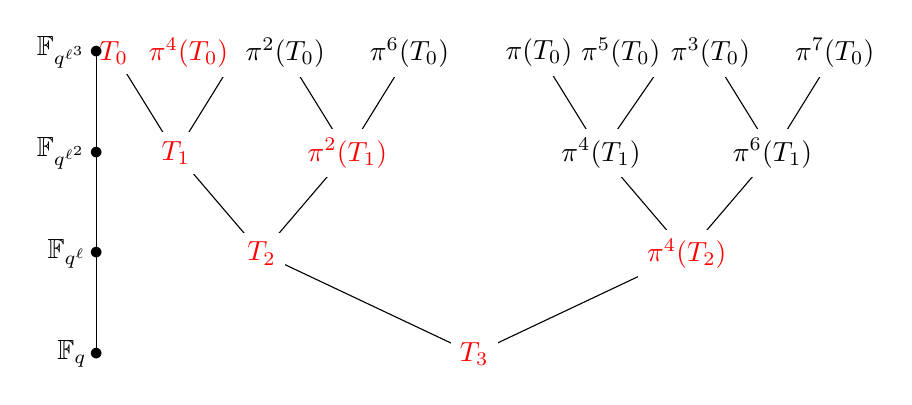
\begin{tikzpicture}[scale=0.3]
        \coordinate (A) at (0,0);
        \coordinate (AB) at (-9,4.25);
		\coordinate (AC) at (9,4.25);
		\draw (A)--(AB);
		\draw (A)--(AC);
		\draw (A) node[fill=white]{$\color{red}{T_3}$};
		

		\coordinate (ABA) at (-12.63,8.5);
		%\coordinate (ABA) at (-11.63,8.5);
		
		\draw (ABA)--(AB);
		
		\coordinate (ABAb) at (-15.26,12.75);
		%\coordinate (ABAb) at (-14.26,12.75);
		
		\draw (ABA)--(ABAb);
		\draw (ABAb) node[fill=white]{$\color{red}{T_0}$};
		
		\coordinate (ABAa) at (-10,12.75);
		%\coordinate (ABAa) at (-9,12.75);
		
		
		\draw (ABA)--(ABAa);
		\draw (ABA) node[fill=white]{$\color{red}{T_1}$};
		\draw (ABAa) node[fill=white][left]{$\color{red}{\pi^4(T_0)}$};%ancien \pi(T)
		
		\coordinate (ACA) at (-5.37,8.5);
		%\coordinate (ACA) at (-6.37,8.5);
		
		
		\draw (AB)--(ACA);
		\draw (AB) node[fill=white]{$\color{red}{T_2}$};
		\coordinate (ACAa) at (-8,12.75);
		%\coordinate (ACAa) at (-9,12.75);
		
		
		\draw (ACA)--(ACAa);
		\draw (ACAa) node[fill=white]{$\pi^2(T_0)$};%ancien \pi^2(T)
		
		\coordinate (ACAb) at (-2.74,12.75);
		%\coordinate (ACAb) at (-3.74,12.75);
		
		
		\draw (ACA)--(ACAb);
		\draw (ACAb) node[fill=white]{$\pi^6(T_0)$};%ancien \pi^3(T)
		\draw (ACA) node[fill=white]{$\color{red}{\pi^2(T_1)}$};% ancien \pi^2(T_2)
		
		\begin{scope}[xshift=18cm]
		\coordinate (ABA) at (-12.63,8.5);
		%\coordinate (ABA) at (-11.63,8.5);

		\draw (ABA)--(AC);
		
		\coordinate (ABAb) at (-15.26,12.75);
		%\coordinate (ABAb) at (-14.26,12.75);
		
		\draw (ABA)--(ABAb);
		\draw (ABAb) node[fill=white]{$\pi(T_0)$};%ancien \pi^4(T)
		
		\coordinate (ABAa) at (-9.7,12.75);
		%\coordinate (ABAa) at (-9,12.75);
		
		
		\draw (ABA)--(ABAa);
		\draw (ABAa) node[fill=white,left]{$\pi^5(T_0)$};%ancien \pi^5(T)
		\draw (ABA) node[fill=white]{$\pi^4(T_1)$};%ancien \pi^4(T_2)
		
		\coordinate (ACA) at (-5.37,8.5);
		%\coordinate (ACA) at (-6.37,8.5);
		
		
		\draw (AC)--(ACA);
		\draw (AC) node[fill=white]{$\color{red}{\pi^4(T_2)}$};%ancien \pi^4(T_3)
		
		\coordinate (ACAa) at (-8,12.75);
		%\coordinate (ACAa) at (-9,12.75);
		
		
		\draw (ACA)--(ACAa);
		\draw (ACAa) node[fill=white]{$\pi^3(T_0)$};%ancien \pi^6(T)
		
		\coordinate (ACAb) at (-2.74,12.75);
		%\coordinate (ACAb) at (-3.74,12.75);
		
		
		\draw (ACA)--(ACAb);
		\draw (ACAb) node[fill=white]{$\pi^7(T_0)$};%ancien \pi^7(T)	
		\draw (ACA) node[fill=white]{$\pi^6(T_1)$};%ancien \pi^6(T_2)	
		\end{scope}
		
		\coordinate (A1) at (-16,0);
		\coordinate (A2) at (-16,4.25);
		\coordinate (A3) at (-16,8.5);
		\coordinate (A4) at (-16,12.75);
		\draw (A1)--(A2)--(A3)--(A4);
		\draw (A1) node{$\bullet$};
		\draw (A2) node{$\bullet$};
		\draw (A3) node{$\bullet$};
		\draw (A4) node{$\bullet$};
		\draw (A1) node[left]{$\mathbb{F}_q$};
		\draw (A2) node[left]{$\mathbb{F}_{q^\ell}$};
		\draw (A3) node[left]{$\mathbb{F}_{q^{\ell^2}}$};
		\draw (A4) node[left]{$\mathbb{F}_{q^{\ell^3}}$};
\end{tikzpicture}

\end{center}
\caption{Subproduct tree}
\end{figure}
\end{frame}


\begin{frame}
\frametitle{Experiments}
The algorithm has been implemented on SageMath v7.1 for the case of $\ell=2$ with the $2$-adic tower construction of [Doliskani-Schost '15].%, the code is available on on github: \url{https://github.com/Hugounenq-Cyril/Two_curves_on_a_volcano}
Here we can see a graph for a curve defined on $\mathbb{F}_{101}$ for which we compute the algorithm in two part for differents  inputs $r$. The interpolation correspond to only one step of interpolation:
%Mettre des belles courbes
\begin{figure}[hbtp]
\centering
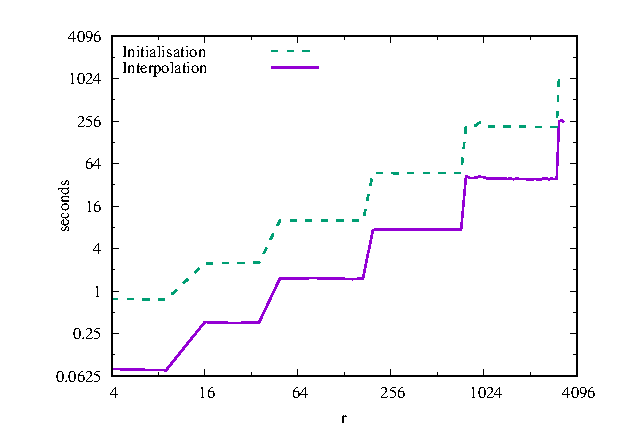
\includegraphics[scale=0.7]{Images/graphe-101-bis.eps}
\end{figure}
\end{frame}


\begin{frame}
\frametitle{Experiments}
Comparisons of execution times (in s) of one interpolation step for various characteristics, for a fixed curve $E$ and increasing $r$.
\begin{figure}[hbtp]
\centering
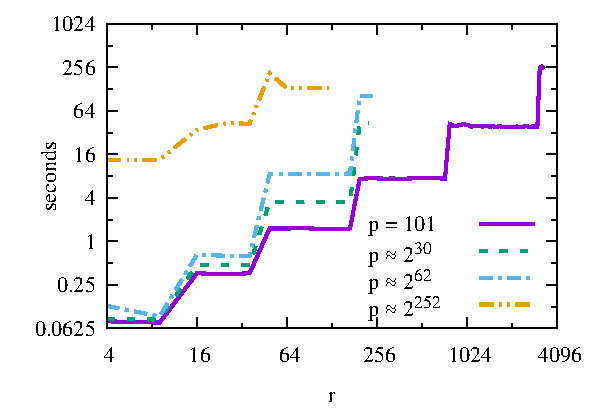
\includegraphics[scale=0.8]{Images/graphe-101-149-269.pdf}
\end{figure}
\end{frame}




\begin{frame}
\frametitle{Conclusion}
\bluebox{Contribution}{
\begin{itemize}
\item A better understanding of the action of the Frobenius endomorphism on isogeny volcanoes. 

\item A faster variant of Couveignes' algorithm.

\end{itemize}
}
\bluebox{Future work}{
\begin{itemize}
\item determine what we can do if we are not on a cyclic crater of a volcano,
\item improve algorithm for curves not on the crater.
\item Atkin!
\end{itemize}}

Code available on GitHub: \url{https://github.com/Hugounenq-Cyril/Two_curves_on_a_volcano}
\end{frame}

\begin{frame} 

\bibliography{Biblio}
\end{frame}

\end{document}

%\begin{frame}
%%\frametitle{Going back to the initial curve}
%{
%%\begin{algorithmic}[1]
%%\STATE $\phi \leftarrow E \rightarrow E/\langle Q \rangle$
%%\STATE $P \leftarrow \phi(P)$
%%\RETURN $P$
%%\end{algorithmic}
%%\begin{algorithmic}[1]
%%\FOR{$i=1$ to $j-1$}
%%\STATE $(P,Q) \leftarrow \textbf{Rectify basis $ \left( P,Q \right)$}$ 
%%\STATE $\phi \leftarrow E \rightarrow E/\langle[2^{j-1}]Q\rangle$
%%\STATE $P \leftarrow \phi(P)$
%%\STATE $Q \leftarrow \phi(Q)/2$
%%\ENDFOR
%%\RETURN $P,Q$
%%\end{algorithmic}
%
%}
%
%\begin{columns}
%\begin{column}[c]{6cm}
%\begin{figure}[hbtp]
%\centering
%\includegraphics[scale=0.4]{Images/Volcan-go-left-premier.eps}
%\end{figure}
%
%\end{column}
%
%\begin{column}[c]{6cm}
%
%\begin{figure}[hbtp]
%\centering
%\includegraphics[scale=0.4]{Images/Volcan-go-left-deuxieme.eps}
%\end{figure}
%\end{column}
%
%\end{columns}
%\end{frame}
%
%
%\begin{frame}
%\begin{columns}
%\begin{column}[c]{6cm}
%\begin{figure}[hbtp]
%\centering
%\includegraphics[scale=0.4]{Images/Volcan-go-right-premier.eps}
%\end{figure}
%
%\end{column}
%
%\begin{column}[c]{6cm}
%
%\begin{figure}[hbtp]
%\centering
%\includegraphics[scale=0.4]{Images/Volcan-go-right-deuxieme.eps}
%\end{figure}
%
%\end{column}
%
%\end{columns}
%\end{frame}
%
%\begin{frame}
%\begin{figure}[hbtp]
%\centering
%\includegraphics[scale=0.8]{Images/Volcan-cratere-rouge-fleche-p-i.pdf} 
%\end{figure}
%\begin{rem}
%We need to give a direction to the horizontal isogeny we choose.
%\end{rem}
%\end{frame}
%
%\begin{frame}
%\bluebox{Benefit of the Frobenius}{
%We can distinguish two paths of length $k$ on the volcano one for each of the "eigenvalues" we have for the Frobenius endomorphism modulo $2^k$.
%}
%
%\begin{figure}[hbtp]
%\centering
%\includegraphics[scale=0.5]{Images/Volcan-cratere-rouge-fleche-lambda.pdf}
%\end{figure} 
%\begin{rem}
%We can always do that if the Frobenius is diagonalizable with two different "eigenvalues" denoted $\lambda_1, \lambda_2$.
%\end{rem}
%\end{frame}
%
%
%\begin{frame}
%\frametitle{Determination of a $2^k$ basis}
%\begin{figure}[hbtp]
%\centering
%\includegraphics[scale=0.4]{Images/Volcan-cratere-noir-chemin-rouge.pdf}
%\end{figure}
%
%\bluebox{Fact}{
%By determining a path of length $k$ on the crater we associate a set of points $P$ of order $2^k$ to this path. Because the path is associated to an $2^k$-isogeny then to the group generated by a primitive $2^k$ torsion point.} 
%\end{frame}
%
%
%\begin{frame}
%\section{Interpolation}
%\frametitle{Interpolation}
%\bluebox{}{
%We want to send point on $E$ that generates an horizontal isogeny associated to $\lambda_1$ on points on $E'$ that generates an horizontal isogeny associated to $\lambda_1$.
%\newline
%Thus we will have to interpolate points:
%\[
%P \rightarrow \mu P'$ with $\mu \wedge 2 =1
%\]
%\[
%Q \rightarrow \nu Q'$ with $\nu \wedge 2 =1
%\]
%}
%\end{frame}
%
%
%\begin{frame}
%\section{Determining a path on the cyclic crater}
%\frametitle{Curves on a cyclic crater}
%To take advantages of the Frobenius we go to an enough higher $2$-torsion where we have $2$ distinct "eigenvalues" for the Frobenius, we denote them by $\lambda_1, \lambda_2$.
%\newline
%\begin{defi}
%We denote by $k$ the least integer such that we have $\lambda_1 \neq \lambda_2 \bmod 2^k $
%\end{defi}
%\newline
%Thus we will work with $2^k$torsion points.
%\end{frame}
%
%
%\begin{frame}
%\frametitle{What about the isogenous curve?}
%\begin{figure}[hbtp]
%
%\centering
%\includegraphics[scale=0.4]{Images/duo-volcan-descendant-noir.pdf}
%\caption{Two volcanoes of $2$-isogeny of elliptic curves related by an odd isogeny}
%\end{figure}
%\end{frame}

%\begin{frame}
%\frametitle{How do we compute generators of the isogeny on the crater?}
%
%\bluebox{Compute $\langle P,Q \rangle = E[2^k]$}{
%\begin{algorithmic}[1]
%\REQUIRE $E: Y^2=X^3+A*X+B$
%\ENSURE $P, Q \in E$ such that $ \langle P,Q \rangle =E[2^k]$
%\end{algorithmic}}
%
%\bluebox{Rectify basis}
%{
%\begin{algorithmic}[1]
%\REQUIRE $\langle P,Q \rangle = E[2^k]$
%\ENSURE $P,Q$ such that $\pi(P)=\lambda_1P,$ $\pi(Q)=\lambda_2 Q, \langle P,Q \rangle = E[2^k]$
%\end{algorithmic}
%}
%\begin{figure}[hbtp]
%\centering
%\includegraphics[scale=0.25]{Images/Volcan-cratere-rectify.eps}
%\end{figure}
%
%
%\end{frame}


%\begin{frame}
%We work with a curve with the following type of $\ell$ structure:\[
%E(\mathbb{F}_q)[2^{\infty}]= \mathbb{Z}/2^{h}\mathbb{Z} \times \mathbb{Z}/2^{j}\mathbb{Z}
%\]with $h \geqslant j+1$
%
%$P$ and $Q$ two points such that : $E[2^{j+1}]=\langle P, Q \rangle$, with \textcolor{red}{$P \in E(\mathbb{F}_q), Q \notin E(\mathbb{F}_q)$}.
%
%\orangebox{Diagonal Matrix}{
%\[
%\pi(P,Q)=\left(\begin{array}{cc}
%1 & 0\\
%0 & q
%\end{array}\right) \bmod 2^{j+1}
%\]
%The points $Q$ associated to a diagonal matrix are the ones such that $\ell^{j}(Q)$ generates a unique $2$-isogeny.
%\newline
%This $2$-isogeny is horizontal if the volcano has a cyclic shaped crater.}
%
%\begin{rem}
%We work with parameters such that \textcolor{red}{$q \neq 1 \bmod 2^{j+1}$}
%\end{rem}
%\end{frame}


%\begin{frame}
%\frametitle{Going further on the crater}
%\begin{defi}[Desired basis]
%We denote by $T_2(E_i)$ the Tate module of $E_i$. We consider $\lambda_1 , \lambda_2$ the two "eigenvalues" of the Frobenius.
%We denote by \[P^i=(P^i_1,P^i_2,..), \pi(P_j^i)=\lambda_1 \cdot P_j^i, P_j^i=2 \cdot P_{j+1}^i \] such that $P_j^i$ is an $2^j$primitive torsion point on $E_i$. 
%We define the same way $Q^i=(Q^i_1,Q^i_2,...)$ with respect to $\lambda_2$.
%Thus we have $T_2(E_i)=(P^i,Q^i)$
%\end{defi}

%\bluebox{Basis intially known}
%{$\langle P_1^i,Q_1^i \rangle $is known with the Frobenius.
%Because we have $\pi(P_k^i)=\lambda_1P_k^1$ and also $\pi(P_k^i+Q_{k-1}^i)=\lambda_1(P_k^i+Q_{k-1}^i)$
%}
%\end{frame}

%\begin{frame}
%\frametitle{Recursive step}
%\begin{prop}
%If we know $Q_j^i \in E_i$ and a point $P \in E_i$ of order $2^k$ such that $\pi(P)=\lambda_1 P \neq \lambda_2 P$ then we are able to determine $Q_{j+1}^{i+1}$. 
%\end{prop}
%
%\begin{proof}
%We consider $\phi: E_i \rightarrow E_i/<2^{k-1}P_k^i>=E_{i+1}$. We have $Q_{j+1}^{i+1}=\phi(\frac{Q_j^i}{2}) $ since we can write  $\frac{Q_j^i}{2}= Q_{j+1}^{i}+ a  P_{1}^{i}$
%\end{proof}
%\end{frame}
